\chapter{Results}

\paragraph{}
In the previous chapter, we delved deeply into the technical implementation of the application which has two goals: to individually display tweets and collect information on the series regarding the interest for each tweet and time deciding the level of interest of each tweet. Using the results from fifteen test users and an analysis of the subsequent data, we will display and explain six graphics. Then, we will interpret the results of the survey. For consistent clarity, we will provide the notation that we are going to use at the beginning of each chapter.

\section{Explanations}

\paragraph{}
As we explain in chapter 3 (method), in order to measure the level of interest and the time of engagement, we created an application, which allows us to do two A/B tests. These two A/B tests, respectively test-time and test-like, are composed by two series each. We have named them test-time-A, test-time-B and test-like-A, test-like-B. To clarify, test-time-A and test-like-A are the calibration tests and that share many similarities. We will present the results acquired by the application, which are based on the number of tweets liked in a series, and the time spend on tweets. The time spent on a tweet is normalized by the number of characters of this tweet. All of the data acquired during the experiment is available on Github [source].

\section{Data}

\subsection{Figure 1}

\paragraph{}
The table [source] gives us two sets of data. Column 1 shows the percentage of people who took more time to do test B than test A. The second column, column 2, shows the percentage of people who liked more tweets in the test B than the test A.\\
When we select the tweets for test-time-B based on the time spent on tweets in test-time-A, we obtain better results when testing for time than when using test-like-B. This demonstrates that 37.5\% of the users spend more time on the series test-time-B than the first test-time-A. However, if we consider the number of tweets liked, we obtain clear results if we take tweets considering the number of tweets liked in the series test-like-A. Our information also demonstrates that 71.4\% of users doing test-like-B liked more tweets than in the series test-like-A.

\begin{figure}[h] 
\centering 
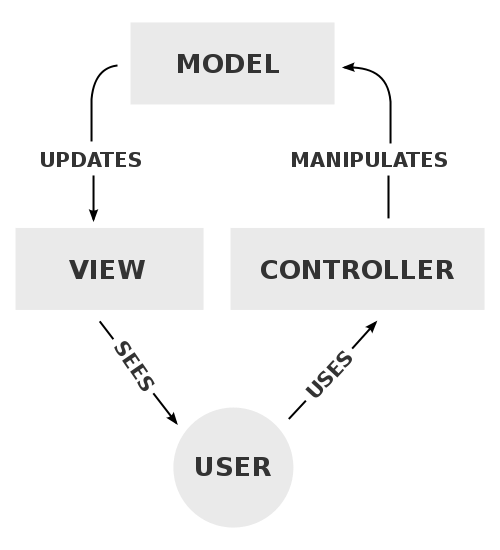
\includegraphics[width=0.5\columnwidth]{technical/MVC} 
\caption[Time spent of Social Media]{This clock shows the distribution of an hour online spent by US people. 16 min are on social network and forum. Source: \cite{s_clock}}
\label{fig:tinder} 
\end{figure}

\subsection{Figure 2}

\paragraph{}
The table [source] gives us the time and 'like' rates that were computed with the formula as demonstrated in ????[source]. Because the test-like-A and test-time-A are the same, it allows us to perform a calibration to see the rates between tests A and tests B.

As demonstrated in column one, for both B tests, people spend on average less time on the second series. However, our information suggests that test-time-B has better results than the other because the difference is 2.51\% when compared to 24.20\% on the other test.
Column two is way better for test-like-B which shows that an increase of 18.52\% in the number of tweets like in average compare to test-like-A. As we did not take in consideration the number of 'likes' in test-time-B, we see this number decrease by 9.14\%.

\begin{figure}[h] 
\centering 
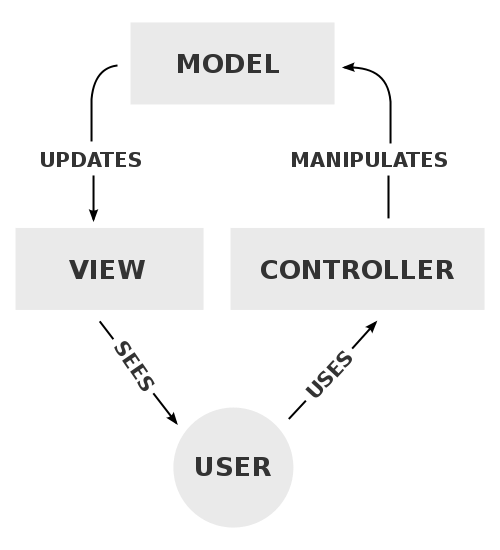
\includegraphics[width=0.5\columnwidth]{technical/MVC} 
\caption[Time spent of Social Media]{This clock shows the distribution of an hour online spent by US people. 16 min are on social network and forum. Source: \cite{s_clock}}
\label{fig:tinder} 
\end{figure}

\subsection{Figure 3}

\paragraph{}
The blue dotted curve in Figure [source] represents the average time spent by all the 15 users on each tweets. The normalized time of the tests A (respectively test-like-A and test-like-A) are given by the value between 1 and 50. From 51 until the end, we have the normalized time spent on tweets of the tests B.
In order to make it more clear, we draw in red the simple moving average of the blue curve. The red curve is obtain with this formula [source]:


We clearly notice that users take more time at the beginning to take a decision. From tweets 1 to 5 people are in average taking double of the time to decide. We do not see  the same augmentation at the beginning of tests B with tweets 51-56.\\
In general, the signal is pretty random with a slight decreasing tendency at the end of each tests, form tweets 30 to 50 and 80 to 100.

\begin{figure}[h] 
\centering 
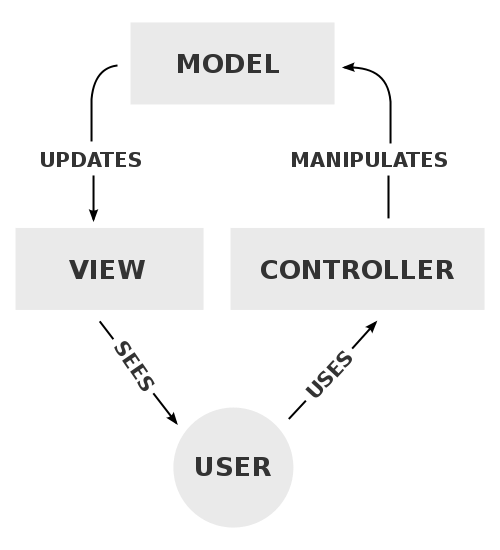
\includegraphics[width=0.5\columnwidth]{technical/MVC} 
\caption[Time spent of Social Media]{This clock shows the distribution of an hour online spent by US people. 16 min are on social network and forum. Source: \cite{s_clock}}
\label{fig:tinder} 
\end{figure}


\subsection{Figure 4}

\paragraph{}
Figure [source] represents as previously, the moving average [source] of the average time spent on tweets in test-like-B (red curve) and tweets in test-time-B (blue curve). We observe that people spend more time in test-time-B than test-like-B. Moreover, after analyzing the data, we can see that the increase of the red curve close to tweet 39 is due a value 20 [source] time superior at the average of the other value.
Moreover, we can see that the blue signal is more random than the red one. Indeed, in series test-like-B, the variation of the signal is equal to 0.4 compare to the 0.9 for the other curve.\\
The decision time is more constant in test-like-B, we can conclude that the decisions are more mechanical than on test-time-B. So,  people are less involve in test-like-B and their engagement time is less important. At the opposite, test-time-B has important variations between tweets decision time, it shows that the engagement is not the same for each tweets but it is in general higher than test-like-B.

\begin{figure}[h] 
\centering 
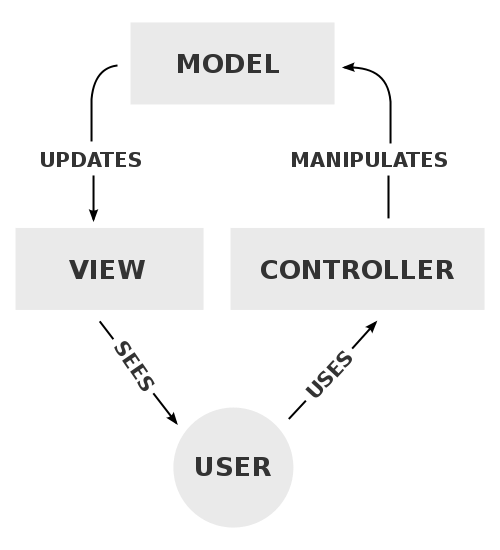
\includegraphics[width=0.5\columnwidth]{technical/MVC} 
\caption[Time spent of Social Media]{This clock shows the distribution of an hour online spent by US people. 16 min are on social network and forum. Source: \cite{s_clock}}
\label{fig:tinder} 
\end{figure}


\subsection{Figure 5}

\paragraph{}
Figure [source], show the moving average of the average of likes that receives tweets during an experience. As previously, tweets 1 to 50 are the test A and tweets 51 to 100 are test-like-B and test-time-B all together.
We can see that the number of likes is almost random during the test. We notice a pick of likes at the beginning of the test B which results from test-like-B and is augmentation of tweets like of 18.52\% [source].
We can conclude that people are classifying tweets until the end of both test. We could have imagine people pressing only L (like) or D (dislike) in order to finish faster.

\begin{figure}[h] 
\centering 
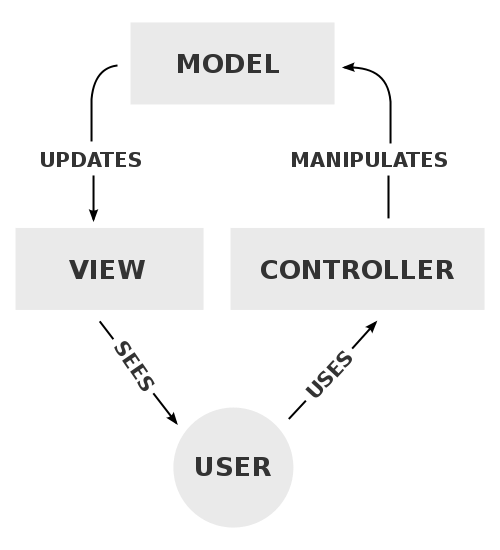
\includegraphics[width=0.5\columnwidth]{technical/MVC} 
\caption[Time spent of Social Media]{This clock shows the distribution of an hour online spent by US people. 16 min are on social network and forum. Source: \cite{s_clock}}
\label{fig:tinder} 
\end{figure}

\subsection{Figure 6}

\paragraph{}
figure [source], gives us the same information that figure [source] but this time we measure the average of likes and not the time. The curve red shows us the moving average of the normalized number of likes in the test-like-B. Respectively, the curve bleu represents the same information in the test-time-B.
We notice that when we select tweets based on the number of likes in test A, we have a higher results than based on the time spent on tweets. This graphic illustres the results of the table [source] which reveal a positive rateLike (18.52\%) for test-like-B and negative (-9.14\% ) for test-time-B.

\begin{figure}[h] 
\centering 
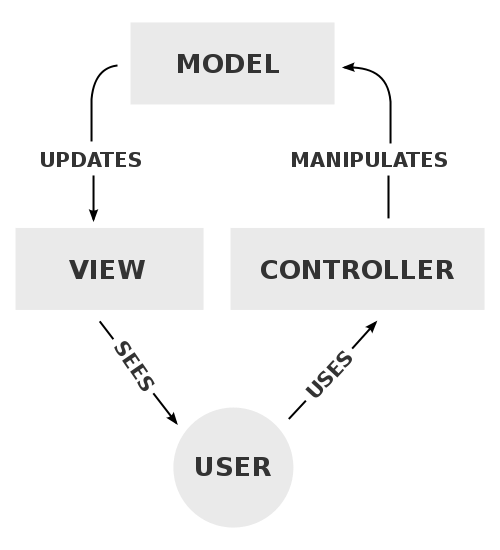
\includegraphics[width=0.5\columnwidth]{technical/MVC} 
\caption[Time spent of Social Media]{This clock shows the distribution of an hour online spent by US people. 16 min are on social network and forum. Source: \cite{s_clock}}
\label{fig:tinder} 
\end{figure}

\section{Survey}

\paragraph{}
After analyzing data from the experiment, we are going to give you the results of the survey that candidate had to fill out at the end of the test. We will give general results about how the 15 people use Twitter. Next, we will analyze the variation of the results between the test A and tests B. The results of the survey are also available on the Github repository [source].

\subsection{General questions}

\paragraph{}
In order to have a better understanding of the results of the experiment, it is interesting to have an average profile of our candidates. To do this profile, we asked three general questions about Twitter, then we can interpreted the average score:
[uneliste]
how often do you use Twitter (1: less than once a week / 5:more than once a day) ?
The average is 3.7, we conclude that our candidates are daily users. They have a good understanding of the service.
Do you usually find the content interesting on twitter ? (1:no /5:yes)
We obtain a result of 3.4 over 5, which is just above the average. Users choose the content that they want on their timeline because they select people that they are following.
Do you usually feel engaged when you are looking at your timeline on Twitter ? (1:no,5:yes)
The result is 3 over 5. On one side, we can conclude that people are not so much engaged on Twitter. On the other side, we can say that people cannot easily measure their engagement on Twitter [source]

In conclusion, our average candidate is a daily twitter user who find the content of his timeline enough interesting to look at it every day. However, his engagement is something unclear and the user spend probably more time on Facebook than Twitter. We will now analyse the results between the test A and test B.


\subsection{Variation between test A and test B}
The table below gives us the variation of engagement, interest and tiredness between test-like-B and test-like-A respectively test-time-B and test-time-A. We see that variation of the interest is in agreement with the previous results [source]. Indeed, the interest decreases of 3.8\% in test-time-B and increase of 26\% in test-like-B. The engagement is almost two time higher in test-like-B and we can put in parallel this engagement and the tiredness of the user after the test-like-B. Then, users are more engagement but the price is significatively high, 38\% more tired. As for test-time-B, the engagement increases of 10\% and candidates are 8.7\% less tired than in test-time-A. \\ \\

\begin{figure}[h] 
\centering 
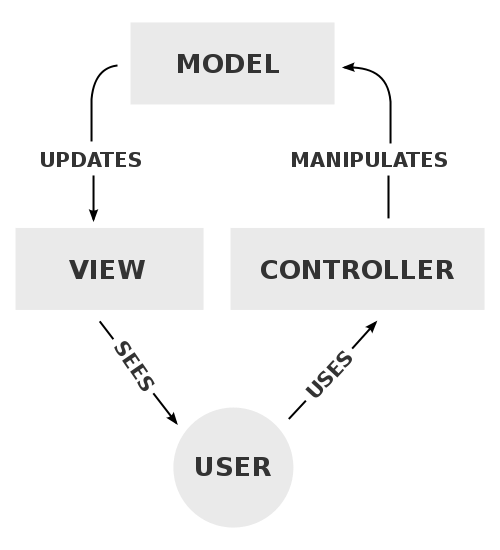
\includegraphics[width=0.5\columnwidth]{technical/MVC} 
\caption[Time spent of Social Media]{This clock shows the distribution of an hour online spent by US people. 16 min are on social network and forum. Source: \cite{s_clock}}
\label{fig:tinder} 
\end{figure}

We finally asked to the candidates: How many tweets are in the series ?\\ 

\begin{figure}[h] 
\centering 
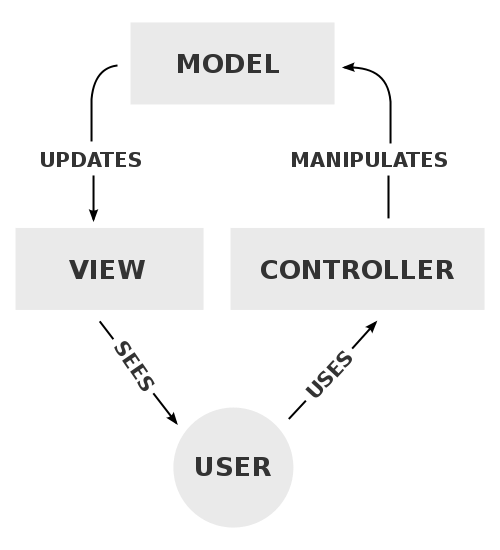
\includegraphics[width=0.5\columnwidth]{technical/MVC} 
\caption[Time spent of Social Media]{This clock shows the distribution of an hour online spent by US people. 16 min are on social network and forum. Source: \cite{s_clock}}
\label{fig:tinder} 
\end{figure}

In general, no matter if it is test-like-B or test-time-B, approximatively 50\% of the candidate answer the correct one: Equal. Now if we consider the statement "More in the first one", we notice that the result is higher for test-time-B. We can link this result to the fact that user are less tired after this test than the user.




